\documentclass[12pt,a4paper]{report} % single-sided
\usepackage[T1]{fontenc}
\usepackage{url}
\usepackage{graphicx}
\usepackage{fancyhdr}
\usepackage{natbib}
\usepackage{multicol}
\usepackage{booktabs}
\usepackage{amsmath}
\usepackage{float}
\usepackage{tikz}
\usetikzlibrary{arrows.meta,positioning,fit,backgrounds}
\usepackage[hidelinks]{hyperref}

% Kent margins (single-sided): 40mm binding edge, others >= 15mm.
\setlength{\oddsidemargin}{14.6mm}
\setlength{\textwidth}{145mm}
\setlength{\topmargin}{-5.4mm}
\setlength{\textheight}{247mm}
\setlength{\headheight}{14.5pt}
\setlength{\headsep}{5mm}
\setlength{\parindent}{0mm}
\setlength{\parskip}{\medskipamount}
\renewcommand\baselinestretch{1.2}
\urlstyle{sf}

\begin{document}
\title{Towards Semantically-Aware End-of-Utterance Detection for Conversational AI Systems}
\author{Jean-Baptiste Azan}

\begin{titlepage}
\vspace*{1mm}
\begin{center}
\Huge Towards Semantically-Aware End-of-Utterance Detection for Conversational AI Systems
\end{center}
\addvspace{30mm}
\begin{center}
\LARGE Jean-Baptiste Azan
\end{center}
\addvspace{35mm}
\begin{center}

\includegraphics[width=50mm]{kent-new.eps}
\end{center}
\addvspace{15mm}
\begin{center}\Large School of Computing\end{center}
\addvspace{25mm}
\begin{center}\Large September 2026\end{center}
\addvspace{25mm}
\end{titlepage}
\setcounter{page}{2}
\pagestyle{empty}

% ---------------------------------------------------------------------------
% Declaration page: paste the completed, dated and signed Access Form here.
% ---------------------------------------------------------------------------
{\Large Declaration}

\vspace{0.75cm}

% TODO: copy and paste the content of the Access Form file from Moodle here,
% dated and signed by you.

\cleardoublepage

\section*{Abstract}

A conversational voice agent has to decide, in real time, when a caller has finished
speaking. On a French medical telephone line that decision is delicate: ending a turn too
early cuts a patient off part-way through a spelled name or a dictated number, while ending
it too late makes the exchange feel slow. Systems that rely on silence alone, a
voice-activity detector and a fixed timeout, hear sound but not meaning, and cut off
utterances that are grammatically incomplete.

This dissertation asks whether adding a lexical, meaning-aware signal improves that
decision, and how the resulting probability should be turned into an endpoint. Two off-the-shelf models, an acoustic end-of-turn detector and a French
language model reading the partial transcript, are fused into one probability; that
probability is calibrated; and the operating point is chosen, in the offline evaluation, from an explicit
interruption-versus-latency cost rather than from a timer. No base model is fine-tuned in the pipeline that produces this result, and no large language
model sits in the decision loop.

On a public French benchmark the fusion raises the per-span AUC from 0.814 to 0.897, a gain of 0.083, with a 95\,\% confidence interval of $[0.063, 0.104]$ and
$p < 3\times10^{-4}$ under a bootstrap resampled by call. Across the
leaderboard, calibration proves a field-wide blind spot: every external detector evaluated
is miscalibrated and none reports it. Validation on 636 production medical calls is
negative, the acoustic branch saturating on 8\,kHz telephony and weak supervision capping
the lexical signal, marking where the approach does not transfer. The contribution is a calibration-first, cost-aware method for composing existing models,
with its limits measured.

\cleardoublepage

\section*{Acknowledgments -> todo}
\vspace{10mm}
% Optional. Thank supervisor and industry partner if you wish.

\clearpage
\pagestyle{fancy}
\fancypagestyle{plain}{%
\fancyhf{}
\renewcommand{\headrulewidth}{0pt}
\renewcommand{\footrulewidth}{0pt}}
\tableofcontents
\listoffigures
\listoftables
\cleardoublepage
\pagestyle{fancy}
\lhead{\nouppercase{\rightmark}}
\rhead{\nouppercase{\leftmark}}
\fancypagestyle{plain}{%
\fancyhf{}
\fancyfoot[C]{\thepage}
\renewcommand{\headrulewidth}{0pt}
\renewcommand{\footrulewidth}{0pt}}
\fancyhf{}
\fancyhead[L]{\slshape \nouppercase{\leftmark}}
\fancyhead[R]{\thepage}
\renewcommand{\headrulewidth}{0.4 pt}
\renewcommand{\footrulewidth}{0 pt}

\bibpunct{(}{)}{;}{a}{}{,}

% ===========================================================================
\cleardoublepage
\chapter{Introduction}
\label{ch:intro}

The rise of large language models (LLMs) has brought with it the voice agent: a system that can
hold a conversation and answer a request, including in demanding fields such as
healthcare. This is the setting for the present project, which was carried out at Tennor,
a company that builds voice agents for healthcare, able to identify patients, answer their
requests, and interact with the software used across the medical sector.

These agents share a design flaw. Because they are built to respond as quickly as
possible, they tend to cut the caller off when a sentence is delivered in several pieces,
for example a spelled-out detail, a telephone number given in blocks, or a pause for
thought. 

A person handles these pauses easily, from the meaning of the words and the
speaker's intonation. A machine that listens only for silence does not. The central
problem of this dissertation is therefore the following: how can the system tell that a
caller has not finished speaking, so that it does not interrupt them, lose information,
and degrade their experience? The decision has to be made in real time after every
silence, and it rests on an uncomfortable trade-off: ending the turn too early talks over
the caller, while waiting too long makes the exchange feel slow.

The title of this dissertation says end-of-utterance; the literature and the benchmark used
here say end-of-turn. They name the same event, the moment a speaker has finished and the
floor is free, and the two are used interchangeably below.

The existing system already separates speech from silence with a voice activity detector
(VAD) and ends the turn after a fixed timeout. It listens to the sound, but not to the
meaning. My idea is to add a semantic signal: a language model reads
the partial transcript and estimates whether the words form a complete utterance. This
signal is fused with the acoustic one into a single probability, that probability is
calibrated, and a stop-or-wait decision is then derived, in the offline evaluation, from an explicit
cost: the price of an interruption set against that of a delay, rather than a simple timer.

Fusing an acoustic signal with a lexical one is not, in itself, new. The contribution of
this project is narrower: a composition of off-the-shelf models, with no joint training and
no large language model in the decision loop; a probability that is validated before it is
trusted; and a decision derived from an explicit cost. The whole
study is grounded in a real case of French medical telephony, with an in-domain dataset
gathered by instrumenting the production system.

How that claim came to be scoped so narrowly is part of the work. When I chose this project
and had it approved, in April 2026, systems fusing an acoustic and a lexical signal existed,
as Chapter~\ref{ch:background} sets out, but none I could find treated its output as a
probability to be calibrated or derived its endpoint from a stated cost. 

The critical review I submitted on 12 June, of a predictive-endpointing paper \citep{zink2024predictive}, ended
by proposing the three things that became this dissertation: the fusion, the calibrated
cost-sensitive decision, and the design that never waits on the transcript. Five days later
LiveKit released a turn detector and an open benchmark that overlapped with the original
angle. Rather than reproduce it, I narrowed the claim to the two things the released systems
still do not do. Their benchmark is also the one this dissertation evaluates on.

On a public French benchmark the fusion raises the per-span AUC from 0.814 to
0.897, a statistically significant gain obtained without fine-tuning either base model.
In domain, however, the same off-the-shelf pipeline does not transfer, and understanding
why turns out to be the more instructive result of the two.

\section{Aims and objectives}
\label{sec:objectives}

I set the project four objectives.

\begin{itemize}
\item \textbf{O1.} Build a modular, real-time endpointing pipeline (VAD, acoustic branch,
lexical branch, fusion, decision) whose decision never waits on the transcript.

\item \textbf{O2.} Fuse an off-the-shelf acoustic detector and a French language model, and
test whether the fusion beats the acoustic model alone on a public benchmark.

\item \textbf{O3.} Calibrate the fused score and choose the operating point from an
explicit cost (interruption against latency) rather than a fixed timeout.

\item \textbf{O4.} Instrument the production agent to build a weakly labelled in-domain
evaluation set, and validate the method in domain.

\end{itemize}


% ===========================================================================
\cleardoublepage
\chapter{Background and Related Work}
\label{ch:background}

\section{The turn problem inside a conversation between two humans}
\label{sec:turntaking}

Turn-taking is the way two speakers alternate in holding the floor. For a machine, the
difficulty is to decide, at every short pause in the exchange, whether to start speaking
because the turn has ended, or to keep waiting because the other party has not finished.
That decision rests on a trade-off that Section~\ref{sec:tradeoff} states formally, and no
setting escapes both of its errors. 

In most dialogue systems the decision is taken from
silence alone: the system waits for a pause of fixed length and then treats the turn as
over. The organisation of turn-taking has been studied since \citet{sacks1974turntaking},
and the rule is simple and fast, but it conflates two very different situations, a
genuine end of turn and a pause in the middle of an utterance, because both present
themselves as silence. In medical telephony this confusion is both frequent and costly: a
patient spelling a name or dictating a number produces silences that are not ends of turn.

These are precisely the cases on which models that listen only to sound fail. 

Having no access to the meaning of the words, they cannot separate a finished sentence from a
spelling sequence or a number still in progress. A perceptual study on French shows that the two channels are not interchangeable
\citep{uro2024perceptive}. Inter-pause units drawn from the REPERE corpus were annotated
for terminality and presented to participants either as audio or as text, with the end of
the unit truncated by up to three prosodic words; participants then judged whether the floor
could be taken. The audio condition allowed a turn end to be anticipated at least three
words before it arrived, the text condition considerably less.

That result ranks the two channels, and ranks them in favour of audio, which is the baseline
this project sets out to improve. What it establishes is separability: the same boundary
judged from sound and from words produces different judgements. Whether the difference
combines into something better than either channel alone is an empirical question, and
Section~\ref{sec:fusionresults} answers it.

\section{Tools and technologies}
\label{sec:tools}

The system reuses several existing components, described briefly here.

Voice activity detection is handled by Silero VAD \citep{silero_vad}, an open-source
package with no accompanying academic publication, which labels each short audio frame as
speech or silence. It is the entry point of the pipeline: it triggers an evaluation at
every transition from speech to silence.

The acoustic end-of-turn estimate comes from Smart Turn v3, a model released by Pipecat
and Daily \citep{smartturn_v3}, likewise without an academic publication and documented
only by its model card and a technical blog post. It uses the encoder layers of Whisper
Tiny \citep{radford2023whisper} with a single linear classification head on top, for
roughly eight million parameters. From the recent audio it produces a probability that the
turn has ended, without reading any text. This project uses version 3.2 in its CPU export.
Versions 3.1 and 3.2 improved the handling of short utterances and robustness to noise,
and the exact version is stated because the reported figures depend on it.

The lexical estimate comes from CamemBERT \citep{martin2020camembert}, a French
BERT-style language model applied to the partial transcript. Unlike the acoustic signal,
it judges completeness from the meaning of the words. Continuous transcription is provided
by a commercial speech recognition service (Azure), which emits partial hypotheses as
speech unfolds.

Evaluation relies on eot-bench \citep{eotbench}, which its authors describe as the first
open collection of genuine human-to-agent turns with aligned audio and textual context,
covering fourteen languages of which French is one. Rather than fixing a single threshold,
the harness sweeps the policy jointly over threshold, action delay and timeout and reports
the frontier between latency and cut-ins. It is an industrial artefact rather than a
peer-reviewed publication, released under Apache-2.0 in June 2026 alongside the LiveKit Turn
Detector v1, three weeks before implementation began here.

One caveat qualifies Chapter~\ref{ch:results}. Its authors omit scalar ranking metrics such
as the area under the receiver operating characteristic curve (AUC) from their comparison
reports, treating them as diagnostic only. This dissertation reports per-span AUC as its
headline figure because the question here is whether a lexical signal improves the
underlying \emph{score}, which a policy sweep conflates with the timing applied on top of
it. Both views are reported throughout.

\section{Calibration and cost-sensitive decision}
\label{sec:calibration-lit}

Neither of the two bodies of method underpinning the decision layer is specific to
turn-taking.

The first is probability calibration. A classifier is calibrated when, among the cases it
assigns a probability of $0.8$, roughly eight in ten are positive. Modern neural networks
are systematically miscalibrated and typically overconfident;
\citet{guo2017calibration} attribute this to model capacity and to training choices such as
batch normalisation, and show that accuracy and calibration can move in opposite directions.
Calibration is therefore not implied by good discrimination: a model can rank correctly, and
so obtain a high AUC, while the values it emits are meaningless as frequencies. 

The standard remedies are post-hoc and monotonic. Platt scaling fits a sigmoid; isotonic regression
\citep{zadrozny2002isotonic} fits an arbitrary non-decreasing step function, more flexible
but hungrier for held-out data \citep{niculescu2005predicting}. Being monotonic, neither
changes the ranking, and so neither changes the AUC: they correct the values, not the
ordering. Calibration quality is measured by the expected calibration error, or ECE
\citep{naeini2015ece,guo2017calibration}, defined in Section~\ref{sec:calibdesign}.

The second is cost-sensitive decision making. Once a probability is trustworthy, where to
act is not a free parameter but a consequence of the relative cost of the two errors:
\citet{elkan2001cost} shows that under an asymmetric loss the operating point follows from
the cost ratio rather than being set by hand. The rule used here decides on the evidence
available at one instant. The richer alternative lets observations accumulate and weighs
acting now against paying to observe more; the canonical formulation is Wald's sequential
probability ratio test \citep{wald1945sequential}, which Chapter~\ref{ch:conclusions}
returns to as future work.

A third strand is relevant to the in-domain dataset rather than the decision. Weak
supervision replaces manual annotation with cheap, noisy labelling heuristics, an approach
systematised by \citet{ratner2017snorkel}. It buys
scale and, in a clinical setting, avoids a person having to listen to call content, at the
cost of label noise that bounds the signal any model can recover from the data. That bound explains the in-domain result of Section~\ref{sec:gold}.

\section{Related work on end-of-turn detection}
\label{sec:related}

Work on end-of-turn detection can be grouped by the signals it uses.

\emph{Purely acoustic} approaches decide from sound, prosody and silence, without reading
the words. They are fast and independent of transcription, but blind to meaning, and so
cut off utterances that are grammatically incomplete. Smart Turn, the baseline of this
project, belongs to this family. A more elaborate member is
\citet{zink2024predictive}, which trains a Conformer to transcribe before an utterance
finishes and reads the decoder's cross-attention at the end-of-sentence token to locate the
endpoint, so no separate language model is needed. It is evaluated offline on pre-segmented
utterances, however, and never inside a running dialogue system, so it is not shown that the
timing it saves survives streaming constraints. That gap shaped the present design.

\emph{Purely lexical} approaches read the transcribed text and judge whether the utterance
is complete. They supply the meaning the acoustic signal lacks, but they inherit a dependency that shapes
both the design of Chapter~\ref{ch:approach} and the failure reported in
Section~\ref{sec:gold}. A lexical branch is only as good as the transcript it reads, and a
streaming transcript is late, unstable and imperfect: partials arrive behind the audio, are
revised as context arrives, and degrade on narrowband telephone speech. Waiting for a stable
transcript buys accuracy with the latency endpointing is trying to save; reading whatever is
available reads a text that may be wrong. Neither horn is free.

\emph{Joint} approaches process audio and text together. FastTurn \citep{fastturn2026} unifies streaming connectionist temporal classification (CTC)
decoding with acoustic features so that a
decision can be taken early from partial observations while semantic cues are preserved.
It performs well but is heavy and presupposes joint training of its components. JAL-Turn
\citep{jalturn2026} combines pre-trained acoustic representations with linguistic features
through a lightweight joint model built on a frozen automatic speech recognition (ASR)
encoder, so that it runs in
parallel with recognition and adds no latency. Unlike FastTurn it does not require the two
modalities to be retrained together, and its labels are extracted automatically from
large-scale dialogue corpora. 

X2-Turn \citep{x2turn2026} goes further, placing a frame-synchronous turn state head
alongside the ASR head on shared streaming features. Phoenix-VAD \citep{phoenixvad2025}
takes the opposite route to the one adopted here, putting a large language model inside the
endpoint decision itself.

On the benchmarking side, the LiveKit detector and test set provide the policy-sweep
evaluation framework this project adopts. Other work remains purely acoustic: endpoint
anticipation \citep{udupa2026anticipation} bypasses ASR to predict a turn ending in
advance, up to roughly 2.5 seconds ahead, so that the rest of the pipeline can be started
sooner. Its object is not the choice of a decision threshold but early prediction, and the
cost it seeks to reduce is the speculative computation wasted when the pipeline is
launched too early and then abandoned.

The closest neighbour is Easy Turn \citep{easyturn2025}, an open-source modular detector
that also integrates acoustic and linguistic information and also positions itself against
Smart Turn. 

Beyond that the two diverge on every axis that matters. Easy Turn trains: its
model is fitted on a purpose-built 1{,}145-hour corpus and predicts one of four dialogue
states, from which a decision is taken by argmax. The present work trains no base model,
fitting only a linear head on frozen embeddings and a four-parameter fusion above it, and
emits a scalar probability rather than a class. 

Easy Turn reports accuracy on its own test set; this work reports on a third-party benchmark in a language subset it did not choose.
And neither Easy Turn nor any system reviewed here reports whether its probability is
calibrated, or connects its operating point to a stated cost. Fusion is done in both; what
differs is that the output is treated as a probability to be validated before a threshold
placed on it can mean anything.

Table~\ref{tab:related} summarises the comparison.

\begin{table}[H]
\centering
\caption[Recent turn-taking systems compared]{Representative recent end-of-turn detection
systems and where this work sits. ``Calib.'' records whether the system reports any
measurement or correction of the calibration of its own output probability.}
\label{tab:related}
\footnotesize
\setlength{\tabcolsep}{3pt}
\begin{tabular}{@{}p{2.2cm}p{2.4cm}p{2.5cm}p{2.8cm}p{1.0cm}p{2.5cm}@{}}
\toprule
System & Signals & Training & Decision rule & Calib. & Evaluation \\
\midrule
Easy Turn (2025) & acoustic + linguistic & trained, 1{,}145\,h & argmax over 4 states & no & own test set \\
Phoenix-VAD (2025) & LLM over text & LLM fine-tuned & LLM in the loop & no & own test set \\
JAL-Turn (2026) & acoustic + linguistic & head only, frozen ASR & fixed threshold & no & multilingual \\
FastTurn (2026) & acoustic + CTC & joint training & early, on partials & no & own test set \\
X2-Turn (2026) & shared ASR features & joint, dual-head & per-frame state & no & own test set \\
Endpoint antic. (2026) & acoustic only & trained & per-horizon threshold & no & anticipation only \\
LiveKit v1 (2026) & text (+ VAD) & trained detector & swept policy & no & 14-language benchmark \\
\midrule
\textbf{This work} & acoustic + lexical & \textbf{frozen bases}; linear head + fusion & \textbf{cost-derived, on a calibrated probability} & \textbf{yes} & French benchmark + medical domain \\
\bottomrule
\end{tabular}
\end{table}

The fusion mechanism itself, combining an acoustic signal with a lexical one, and the
latency-versus-cut-in framing are not new, and this project claims to have invented
neither. The field is moving fast enough that every one
of the seven systems in Table~\ref{tab:related} was published in the eleven months to
August 2026, and the most recent of them appeared three weeks before this chapter was
written.

\section{The gap addressed}
\label{sec:gap}

Three gaps emerge from this review. Almost all of the work above appeared after this
project was scoped (Chapter~\ref{ch:intro}), so these are the gaps that remain \emph{after}
that shift, not the ones the project was originally scoped against.

First, none of the systems reviewed reports an explicit
calibration of its probability, neither an expected calibration error nor any
recalibration, and none relates its decision threshold to a cost of interruption against
latency: eot-bench sweeps thresholds and some vendors expose confidence scores, but the
probability itself is neither measured nor corrected, so a chosen threshold has no precise
meaning. 

Second, Table~\ref{tab:related} shows the field moving steadily towards larger jointly
trained systems. The opposite end of the design space, where frozen components are merely
composed, is little studied.
Third, the French medical telephony domain, where semantically incomplete utterances
(spelling, digits, dates) are both frequent and consequential, is not addressed. These
are the three gaps this dissertation sets out to close.


% ===========================================================================
\cleardoublepage
\chapter{Design and Trade-Off Analysis}
\label{ch:approach}

\section{The central trade-off: latency against interruption}
\label{sec:tradeoff}

Every decision in this chapter serves the trade-off introduced in
Chapter~\ref{ch:background}, which I state formally here. At each micro-pause, ending the
turn too early cuts the patient off, an interruption of cost $C_{\mathrm{cut}}$, while
waiting too long delays the reply, latency of cost $C_{\mathrm{lat}}$. Improving one
degrades the other, and no setting escapes both. Designing the system therefore comes down to deciding, at every instant, which side of that
trade-off to sit on, and deciding it for a stated reason. Each section below sets out one decision and the
trade-off it resolves.

\section{Which data trains, and which data validates}
\label{sec:datastrategy}

The project started from the assumption that Tennor's production transcripts would be the
training data and that the evaluation would be built around them. I reversed that in late
July, and because the reversal shaped everything downstream it belongs here rather than in
the implementation chapter.

Licensing forced it, and so did the labels. The eot-bench harness is Apache-2.0 and its
dataset CC-BY-4.0, both usable for research and derivative work; the production data is
personal data that cannot leave Tennor's infrastructure at all
(Appendix~\ref{app:ethics}), so anything built on it alone would be a result nobody else
could check. The two also differ in what they can support: the benchmark carries
human-verified turn boundaries, while the production set is labelled by weak supervision,
from whether the caller resumed speaking, which is cheap and scalable but noisy by
construction.

So I inverted the roles. The public benchmark carries the headline experiments (fusion,
calibration, cost), and the production data becomes an in-domain validation set, asked
only the narrower question of whether the method transfers.

The cost of that inversion is real and worth naming. The headline result is obtained on
generic French rather than on medical French, so the domain that motivates the project is
not the domain the main claim is measured on. And a weakly labelled validation set can only
return a weak answer, which is precisely what Chapter~\ref{ch:results} reports. What it
buys is that every headline number in this dissertation can be reproduced by anyone with a
Hugging Face token, and none of them rests on data that nobody outside Tennor can see.

\section{Late fusion rather than a jointly trained model}
\label{sec:latefusion}

The first modelling decision was how to combine the acoustic and the lexical signal. One
option is a single model trained jointly on audio and text. It can be more accurate,
because it learns the interactions between the two modalities, but it is heavier to run, it
demands aligned joint training data, and it locks both signals inside one box that cannot
be replaced piecemeal. The alternative, and the one I took, is late fusion: each signal
comes from an independent off-the-shelf model, and only their combination is learned.

I may lose some accuracy that way. What I gain is modularity, since each component can be
swapped on its own, along with speed and simplicity, which matches the constraint the
project set itself of composing existing models without retraining them.

\section{The lexical model: frozen embeddings rather than fine-tuning}
\label{sec:frozen}

The lexical signal can be obtained in two ways. CamemBERT can be fine-tuned on Tennor
medical French, which produces a \emph{medical-fitted} model closely adapted to that domain
but out of distribution on generic French, where it degrades the decision rather than
improving it. Section~\ref{sec:fusionresults} measures this. Or CamemBERT can be left frozen and used purely as a
feature extractor, with a small classifier on top, which generalises better and cannot
overfit the way a fine-tuned encoder can.

The two are named for the data they were fitted on in the chapters that follow:
\emph{benchmark-fitted} is the frozen encoder under a head fitted on the benchmark, and
\emph{medical-fitted} is the encoder fine-tuned on medical French. I kept both, for
different paths. The frozen encoder with a head fitted on the benchmark,
\emph{benchmark-fitted} in the tables of Chapter~\ref{ch:results}, serves the benchmark
evaluation. The medical-fitted model serves the in-domain path and the live demonstration,
where medical French is what it will actually see.

\section{A decision that never blocks on the transcript}
\label{sec:nonblocking}

One constraint governs the whole pipeline: the decision has to stay fast, while streaming
transcription can and does fall behind. I could wait for the most complete transcript available, paying added latency and risking a
stall, or read whatever partial transcript exists at the instant of the decision, as a
snapshot, accepting that it may lag the audio.

I took the second. The decision never waits on the recogniser: the transcript is read as
whatever snapshot exists at that instant. The two model calls are issued concurrently and
both are awaited, so the added latency is the slower of the two rather than their sum. Added latency is bounded by construction,
and the price is a text that is sometimes slightly incomplete. That is acceptable, because the
acoustic signal is always available and the fusion degrades gracefully when the lexical
branch has little to say. This is the design answer to the ASR dependency set out in
Section~\ref{sec:related}.

\section{The form of the fusion}
\label{sec:fusionform}

The fusion takes two forms, and the difference between them runs through the rest of this
dissertation. A rule-based form applies a bilateral veto and then a fixed
average; it needs no data to fit, so it was the committed deliverable and it is what the
system runs (Section~\ref{sec:fusionimpl}). The two operations are sequential rather than
combined: the veto is a gate, and when either signal falls below its threshold the decision
is to wait and the average is never computed. Only when both signals clear the gate are
they averaged, and the result is then mapped onto how much trailing silence to demand. A learned form fits the combination, and it is
the one every result in Chapter~\ref{ch:results} is measured on. The rule form is described
with the implementation because it is an engineering artefact; the learned form is set out
here because its shape is a design decision.

In the learned form the two probabilities are combined by logistic regression on
$p_{\mathrm{ac}}$, $p_{\mathrm{lex}}$ and their product. With weights $w_0 \dots w_3$,
\begin{equation}
z = w_0 + w_1 p_{\mathrm{ac}} + w_2 p_{\mathrm{lex}} + w_3\, p_{\mathrm{ac}} p_{\mathrm{lex}},
\qquad
p_{\mathrm{raw}} = \sigma(z) = \frac{1}{1 + e^{-z}} .
\label{eq:fusion}
\end{equation}
Here $p_{\mathrm{ac}} \in [0,1]$ is the probability of end of turn produced by the acoustic
model and $p_{\mathrm{lex}} \in [0,1]$ the one produced by the lexical model, both read at
the same micro-pause; $z$ is the linear score they are combined into; $\sigma$ is the
logistic function; and $p_{\mathrm{raw}} \in [0,1]$ is the fused probability before any
calibration. There are four weights because the model has four terms and no more: an
intercept $w_0$, one weight per input signal, and $w_3$ on their product.

This form contains the rule-based one as a special case. The fixed average
$0.5\,p_{\mathrm{ac}} + 0.5\,p_{\mathrm{lex}}$ is Equation~\ref{eq:fusion} with
$w_0 = 0$, $w_1 = w_2 = 0.5$ and $w_3 = 0$: the same shape, with the weights set by hand
instead of fitted, and with the interaction term switched off. What fitting them adds is
visible in the values Section~\ref{sec:fusionresults} reports: the lexical branch receives
roughly $2.2$ times the weight of the acoustic one, so the equal split the rule form
assumes is not what the data supports. The veto and the silence ladder run the other way:
they are gating structure that Equation~\ref{eq:fusion} has no counterpart for. The interaction
term $p_{\mathrm{ac}} p_{\mathrm{lex}}$ lets the model treat the case where both signals
agree as different from the sum of their separate contributions, which a purely additive
form cannot represent. 

I preferred logistic regression to richer combinations because it is light, its weights stay interpretable, so one can read off which of the
two signals carries more of the decision, and its output is a probability that can then
be calibrated. The fusion itself is small enough not to memorise a dataset of roughly a thousand spans,
though the lexical head above it is not: a logistic layer on 768-dimensional frozen
embeddings carries 769 parameters against some eight hundred training rows per fold, which
is why every lexical and fusion figure in Chapter~\ref{ch:results} is reported
out-of-fold. The weights are fitted by cross-validation with folds split by
call, so that no call appears in both training and test.

\section{Calibrating before deciding}
\label{sec:calibdesign}

A structural decision is to treat the probability the system produces as a quantity that
must be calibrated before it is used. The reason is direct. The final decision compares
that probability against a threshold derived from a cost, and the comparison only means
anything if the probability corresponds to a real frequency. As Section~\ref{sec:calibration-lit}
sets out, a poorly calibrated model can rank cases correctly and still be systematically
overconfident, which distorts any threshold placed on it.

Calibration is done by isotonic regression, fitting a monotonic $g$ on a held-out split to
minimise $\sum_i (g(p_i) - y_i)^2$. Because $g$ is monotonic it leaves the ordering of
predictions untouched, so the AUC does not move, and only the probability values are corrected. Quality is measured by the expected calibration error,
\begin{equation}
\mathrm{ECE} = \sum_{b} \frac{n_b}{N} \, \bigl| \mathrm{acc}_b - \mathrm{conf}_b \bigr| ,
\label{eq:ece}
\end{equation}
The predictions are sorted into bins $b$ by the probability they carry. For each bin,
$n_b$ is the number of predictions it holds, $N$ the total number of predictions,
$\mathrm{conf}_b$ the mean probability claimed within the bin, and $\mathrm{acc}_b$ the
proportion of those cases that turned out positive. The ECE is therefore the average gap
between claimed confidence and observed frequency, each bin weighted by how many predictions
fall into it. The cost of the approach is that it consumes held-out data and can
overfit on small sets, which I limit with a held-out split rather than reusing the fitting
data.

\section{Deciding from a cost rather than a fixed timeout}
\label{sec:costdesign}

The last decision is the stopping rule. The existing system stops after a fixed silence,
500\,ms say: simple, but arbitrary, and identical in every situation. Instead I choose the
operating point from the trade-off of Section~\ref{sec:tradeoff}. Given the cost ratio
\begin{equation}
\lambda = \frac{C_{\mathrm{cut}}}{C_{\mathrm{lat}}} ,
\qquad
\text{choose the policy minimising}
\quad
\lambda \cdot (\text{cut-in rate}) + (\text{latency}) .
\label{eq:cost}
\end{equation}


The units are easily lost. The cut-in rate is a fraction and the latency is in seconds, so
$\lambda$ is itself measured in seconds: $\lambda = 10$ says one interruption costs as much
as ten seconds of extra waiting, not that it is ten times worse than a delay. 

The operating point is then a consequence of a stated preference rather than a number fixed in advance.
Equation~\ref{eq:cost} is the only form of the rule used here: the policy minimising the
combined cost is selected directly, with no closed-form threshold derived from $\lambda$. A richer variant would fold the elapsed silence into the probability and
decide sequentially, in the spirit of \citet{wald1945sequential}. I built it and it did not
improve on the swept frontier (Section~\ref{sec:negative}), so the calibrated single-instant rule stands, and the full sequential formulation is left to Chapter~\ref{ch:conclusions}.


% ===========================================================================
\cleardoublepage
\chapter{System Architecture and Implementation}
\label{ch:implementation}

\section{A modular architecture behind interfaces}
\label{sec:architecture}

The system is a Python package organised into modules, each behind an abstract interface,
so that a component can be replaced without touching the rest
(Figure~\ref{fig:architecture}). There is an audio source
(\texttt{AudioSource}), a voice activity detector (\texttt{VAD}), a speech recogniser
(\texttt{ASR}), the two end-of-turn branches (\texttt{AcousticEOU} and
\texttt{LexicalEOU}), the fusion (\texttt{Fusion}) and the endpoint controller. This
follows directly from the late-fusion choice of Section~\ref{sec:latefusion}: the
recogniser or the detector can be exchanged, a client to an existing microservice in place
of the in-process model, without the decision logic changing at all.

The decision core is isolated from transport in a per-call session,
\texttt{EouSession}. The session takes raw 16\,kHz mono audio and the latest partial
transcript, and emits a decision at each micro-pause. It is driven by an \texttt{Orchestrator}, which owns an audio source and a recogniser for
the demonstrations and the evaluation harness, and by the WebSocket service, which drives a
session directly.
Both reach the same code, so there is one decision path and not two.

The session carries an explicit statefulness contract, which matters in production:
the heavy models may be shared across concurrent calls, but the VAD holds state and must be
instantiated per session.

\section{The real-time path}
\label{sec:realtime}

The audio source emits frames of 512 samples at 16\,kHz, that is 32\,ms. In production the
transport does not respect that framing, since telephony delivers 20\,ms frames, so the
session accepts a chunk of arbitrary length and re-frames it internally to the fixed size
the VAD expects. Each frame is written to a ring buffer holding the last eight seconds of
signal, passed to the recogniser, and labelled speech or silence by the VAD. When a
speech-to-silence transition lasts beyond 200\,ms, an evaluation is triggered. That is the
micro-pause at which the system decides to end the turn or to wait, and an internal latch
guarantees it fires at most once per turn.

\begin{figure}[H]
\centering
\resizebox{\textwidth}{!}{%
\begin{tikzpicture}[
  font=\small,
  box/.style={draw=black!60, rounded corners=1.5pt, align=center,
              minimum height=9mm, inner xsep=2.5mm, inner ysep=1.5mm},
  fl/.style={-{Stealth[length=2mm]}, draw=black!60},
  sn/.style={-{Stealth[length=2mm]}, draw=black!60, dashed}]

\node[box] (src)  at (0,0)      {Audio source\\\footnotesize 512 samples / 32\,ms};
\node[box] (asr)  at (0,2.0)    {ASR (Azure)\\\footnotesize interim hypotheses};
\node[box] (ring) at (0,-2.0)   {Ring buffer\\\footnotesize last 8\,s};
\node[box] (vad)  at (4.3,0)    {VAD\\\footnotesize speech / silence};
\node[box] (gate) at (8.2,0)    {Micro-pause\\\footnotesize silence $>$ 200\,ms};
\node[box] (ac)   at (12.6,1.6) {Acoustic branch\\\footnotesize Smart Turn v3};
\node[box] (lex)  at (12.6,-1.6){Lexical branch\\\footnotesize CamemBERT};
\node[box] (fus)  at (16.9,0)   {Fusion\\\footnotesize \texttt{RuleFusion}};
\node[box] (ep)   at (20.9,0)   {Endpoint\\\footnotesize controller};
\node      (out)  at (24.2,0)   {\textbf{END} / \textbf{WAIT}};

\draw[fl] (src) -- (vad);
\draw[fl] (src) -- (asr);
\draw[fl] (src) -- (ring);
\draw[fl] (vad) -- (gate);
\draw[fl] (gate) |- (ac);
\draw[fl] (gate) |- (lex);
\draw[fl] (ring) -| (ac);
\draw[sn] (asr)  -| (lex) node[midway, above, font=\footnotesize] {snapshot, never awaited};
\draw[fl] (ac) -| (fus);
\draw[fl] (lex) -| (fus);
\draw[fl] (fus) -- (ep);
\draw[fl] (ep) -- (out);

\begin{scope}[on background layer]
\node[draw=black!35, dashed, rounded corners=2pt, fit=(ac)(lex),
      inner sep=3.5mm, label={[font=\footnotesize, black!55]below:%
      concurrent, in an executor}] {};
\end{scope}
\end{tikzpicture}}
\caption[Pipeline architecture]{The decision pipeline. Every frame feeds the ring buffer,
the recogniser and the VAD. A speech-to-silence transition beyond 200\,ms triggers an
evaluation, in which the two branches run concurrently off the event loop. The lexical branch reads the latest partial transcript as a snapshot, so the decision never waits on
the recogniser; both model calls are awaited, and the added latency is the slower of the
two. The fusion shown is \texttt{RuleFusion}, the variant the system runs; the learned
form of Equation~\ref{eq:fusion} substitutes behind the same interface but is evaluated
offline only.}
\label{fig:architecture}
\end{figure}

The session keeps two clocks. Silence duration is
measured on an audio-sample clock, advanced by the frame duration, so a given recording
always produces the same timing regardless of how fast the machine runs. Wall-clock time is
used for one thing only: measuring how long the models took. A system timing silence by wall clock would behave differently on a loaded machine and on an
idle one, and a replayed clip would not reproduce its own earlier result. This does not
affect Chapter~\ref{ch:results}, whose figures come from stored predictions; it matters for
the live pipeline and the clip-replay harness.

At the moment of evaluation the acoustic and lexical branches are computed concurrently,
off the event loop in an executor, so that incoming frames continue to be processed. The partial transcript is read as a local snapshot and never awaited. That is the
non-blocking property of Section~\ref{sec:nonblocking} in concrete terms: the recogniser is
off the critical path. The two model calls themselves are both awaited, so the added latency
is $\max(\text{acoustic}, \text{lexical})$ and not their sum, and no timeout guards the
lexical future.

\section{The two branches and the recogniser}
\label{sec:branches}

The acoustic branch applies Smart Turn v3 (version 3.2, CPU ONNX export) to the last eight
seconds of the ring buffer and returns a probability that the turn has ended. The lexical
branch applies CamemBERT to the latest partial and returns a completeness probability. The
two variants of Section~\ref{sec:frozen} sit behind the same interface, frozen embeddings
with a classifier for the benchmark and the fine-tuned model for the domain and the live
demonstration. A French heuristic guard (\texttt{FrenchSemanticEOU}) complements the model
on the hard cases, detecting a spelling sequence still in progress, digits, and function
words in final position.

Transcription reuses the production Azure service, with the same language and audio format.
The one non-invasive addition is that it subscribes to the interim hypotheses as well as
the final results, and those feed the lexical branch. Production itself is unchanged.

\section{Fusion and the endpoint controller}
\label{sec:fusionimpl}

\texttt{RuleFusion}, one of the two implementations behind the \texttt{Fusion} interface,
applies a bilateral veto: if either signal falls below 0.25, that is, if either branch clearly reads
mid-turn, the system waits. If both exceed 0.85 it endpoints immediately. Otherwise it
averages the two and hands the result on. \texttt{LogisticFusion} substitutes for it without the
calling code changing. It implements Equation~\ref{eq:fusion} with one addition: a fifth
term on the elapsed silence, normalised by the maximum-silence limit. The benchmark
experiments of Chapter~\ref{ch:results} use the four-parameter form of
Equation~\ref{eq:fusion} without that term, so that the reported gain is attributable to
the two probability signals alone and not to timing information the acoustic baseline never
receives.

One boundary should be drawn here. The learned fusion and the cost rule were staged from
the outset, with the rule-based fusion as the committed deliverable, and neither reached the
running path: \texttt{LogisticFusion} is instantiated nowhere outside a unit test, and no
cost ratio appears anywhere in the runtime package. 

The data strategy of Section~\ref{sec:datastrategy} then fitted both the fusion and the calibrator on generic
French, and Section~\ref{sec:fusionresults} measures what a component fitted on the wrong
domain costs. What the running system demonstrates is the pipeline, its real-time and
non-blocking behaviour, and the capture that produced the in-domain set; the decision layer
of Chapter~\ref{ch:results} is established offline on stored predictions, and carrying it
across is deliberately not claimed here.

The endpoint controller then converts confidence into a duration. Rather than a single
threshold it maps confidence onto how much trailing silence is demanded: 200\,ms above
0.85, 600\,ms above 0.5, 1200\,ms below. Confidence therefore buys speed, and a hesitant
score is made to wait longer rather than being refused outright.

Above all of that sits a hard limit at 2000\,ms, which deliberately overrides the veto. A
caller who genuinely stopped mid-sentence, and whose text will never look complete, would
otherwise be held indefinitely by the lexical branch. This is the one place where the design accepts a wrong cut over an unbounded wait. The
reasoning is about failure modes: an interruption is recoverable in conversation, silence
from the agent is not.

\section{Demonstrations and evaluation tooling}
\label{sec:tooling}

Two demonstrations drive the same core. One runs at the command line, from the microphone or
a wav file replayed as a stream; the other runs in the browser. Both print, at each
decision, the acoustic, lexical and fused probabilities, the decision taken, the observed
silence and the compute latency.

Evaluation rests on two tools: a local harness that replays labelled clips and computes
accuracy, false positives, false negatives and latency, and an adapter that plugs the fusion
into the eot-bench protocol so it can be compared with other systems on identical metrics.

The in-domain scoring path did not survive that route, and the reason cost me a day: the
harness reads audio through the Hugging Face \texttt{Audio} feature, which now requires
\texttt{torchcodec}, which does not load against \texttt{ffmpeg}~8. Rather than pin the
toolchain backwards, a standalone scorer reads the caller wav files with \texttt{soundfile}
and scores each pause with the same models and fold splitting. It produces the figures of
Section~\ref{sec:gold}.

\section{Production instrumentation}
\label{sec:instrumentation}

To build the in-domain set, the production system was instrumented. Capture is gated behind
an organisation-level feature flag. When active, the system records at each micro-pause the
caller-side text only, the trajectory of the recogniser's interim hypotheses, timestamps, a
reference to the audio, and resume or interruption flags. Labels come from weak supervision
with no manual annotation: a pause followed by the caller resuming is a hold, a pause
followed by the agent replying without a resume is an end of turn.

The resulting set is 709 calls placed on a single production organisation, of which roughly
four in five are genuine inbound calls and the rest calls made by internal testers to the
same line. Of those, 636 contribute at least one scored decision pause.
Names, first names and ages are masked in the retained transcripts, and the data stays
within Tennor's infrastructure. Because caller audio is retained and linked to a call identifier, it remains
personal data and is treated as such throughout. Appendix~\ref{app:ethics} sets out the
governance in full.

\section{Testing and verification}
\label{sec:testing}

The system is covered by 45 automated tests, exercising the VAD, the ring buffer, the fusion
and endpoint logic, the lexical rules, the types and the metrics. Integration tests that
need heavy models, credentials or audio hardware skip themselves when those are absent, so
the suite runs anywhere. Every result reported in Chapter~\ref{ch:results} has a
documented command that reproduces it, listed in \texttt{reproduce.md} in the submitted
code corpus.


% ===========================================================================
\cleardoublepage
\chapter{Results and Evaluation}
\label{ch:results}

\section{Evaluation protocol}
\label{sec:protocol}

Evaluation runs through the eot-bench harness on the French subset: 400 turns and
1{,}054 silences, of which 400 are ends of turn and 654 are holds. Each of those silences is one micro-pause in the sense of
Section~\ref{sec:realtime}: one moment at which the system must decide. The harness sweeps
the endpointing policy and reports two measures. Per-span AUC says how well a model tells a
silence that ends a turn from one that is only a pause. The latency and cut-in frontier says
how long the system waits, and how often it speaks over a caller who has not finished. 

Take one silence that ends a turn and one that
does not. The per-span AUC is the probability that the model scores the first higher. 0.5 is
a coin flip, 1.0 is a perfect ordering. All lexical and fusion figures are cross-validated with folds split by call,
so no call appears in both training and test.

One methodological point conditions the comparisons. Three of the systems decide as the transcript
arrives: the streaming recognisers Soniox, AssemblyAI and OpenAI GPT-Realtime 2. They cannot
be scored on per-span AUC, because they score at a different moment from the one evaluated
here. Their latency is reported and their AUC left out, since the number would not be
comparable. 

\section{Fusion against the acoustic baseline}
\label{sec:fusionresults}

Table~\ref{tab:fusion} gives AUC and latency, the latter at a 5\,\% and then a 10\,\%
cut-in budget.

\begin{table}[H]
\centering
\caption[Fusion results on the French benchmark]{Fusion results on the public French
benchmark (eot-bench, 1{,}054 silences). \emph{Benchmark-fitted} means the lexical head was
fitted on the benchmark itself, cross-validated with folds split by call;
\emph{medical-fitted} means the lexical model was fine-tuned on Tennor medical French and
applied here unchanged. The lexical branch was scored per span but never run through the policy sweep on its own,
so it carries no latency figure. TF-IDF is term frequency-inverse document frequency, STT is
speech-to-text.}
\label{tab:fusion}
\begin{tabular}{@{}lccc@{}}
\toprule
Model & AUC & Latency @ 5\,\% & @ 10\,\% \\
\midrule
Acoustic only (Smart Turn v3) & 0.814 & 873\,ms & 608\,ms \\
Lexical only (benchmark-fitted) & 0.845 & --- & --- \\
\midrule
Fusion, medical-fitted lexical & 0.789 & 850\,ms & 659\,ms \\
Fusion, benchmark-fitted TF-IDF & 0.872 & 759\,ms & 548\,ms \\
\textbf{Fusion, benchmark-fitted CamemBERT} & \textbf{0.897} & \textbf{715\,ms} & \textbf{510\,ms} \\
\midrule
ultraVAD & 0.817 & 846\,ms & 613\,ms \\
LiveKit v1-mini (commercial) & 0.884 & 798\,ms & 541\,ms \\
Deepgram Flux (commercial) & 0.915 & 676\,ms & 353\,ms \\
LiveKit v1 (commercial) & 0.937 & 635\,ms & 376\,ms \\
Soniox (streaming STT) & n/a & 557\,ms & 463\,ms \\
\bottomrule
\end{tabular}
\end{table}

Fusion lifts the AUC from 0.814, for the acoustic model, to 0.897: a gain of 0.083. That is the comparison the objectives are stated against,
but not the whole picture. The lexical branch alone reaches 0.845, so what fusion adds over
the better of its two inputs is 0.052, not 0.083. The first number says what the deployed system
would gain, the second whether combining the signals beats taking the stronger one.

A gain is only a contribution if it can be shown statistically, so the data was resampled
by call, three thousand times. The 95\,\% confidence interval on
the gain is $[0.063, 0.104]$; no resample produced a non-positive gain, so $p < 1/3000$, which is the finest bound three
thousand resamples can support. Resampling by
call rather than by silence matters, because silences from one call are not
independent and treating them as such would inflate the significance. The gain is not noise.

The fitted weights are worth reporting, since Section~\ref{sec:fusionform} claims
interpretability as a reason for choosing this form. Averaged over the five folds they are
$w_0 = -3.59$, $w_{\mathrm{ac}} = 1.95$, $w_{\mathrm{lex}} = 4.29$ and
$w_{\mathrm{inter}} = 1.22$, with a standard deviation across folds of at most $0.21$. The
lexical branch therefore carries about $2.2$ times the weight of the acoustic one, which
agrees with the two branches scored separately and is the opposite of what the framing of
this project assumed.

The bottom of the table sets the condition under which fusion helps at all. The lexical
signal only helps when it is in distribution. The medical-fitted model, applied to the
generic French of the benchmark, degrades the decision to 0.789, below the acoustic baseline
it was meant to improve. Fusion
is not beneficial in itself. It is beneficial on condition that the lexical model matches
the data, and that condition bounds where this method can be deployed.

The comparison against the other systems needs care. The table adds ultraVAD, an
open-source detector that scores on audio alone, like Smart Turn. At 0.817 it edges past the
acoustic baseline. That is worth recording, because it is the only comparator here that is
neither commercial nor part of this project. At 0.897 the fusion sits above it and above
LiveKit v1-mini (0.884), but below Deepgram Flux (0.915) and LiveKit v1 (0.937). It does not
beat the strongest commercial detectors on AUC, and the margin against v1-mini is too small
to claim a win there either.

On latency it trails as well: 715\,ms against 557\,ms for Soniox and 635\,ms for LiveKit v1
at a 5\,\% budget. Deciding at a micro-pause rather than as the text arrives is a real cost,
and a deliberate consequence of not blocking on transcription
(Section~\ref{sec:nonblocking}). It is not the whole explanation, though: two of the three
streaming services are slower still, AssemblyAI at 822\,ms and GPT-Realtime 2 at 837\,ms.

Figure~\ref{fig:pareto} extends the two budgets of the table to the whole frontier.
The fusion curve sits below the acoustic one across the entire range, so the gain is not an
artefact of the operating points chosen for reporting. It also sits above the LiveKit curve
throughout, so neither is the shortfall.

\begin{figure}[H]
\centering
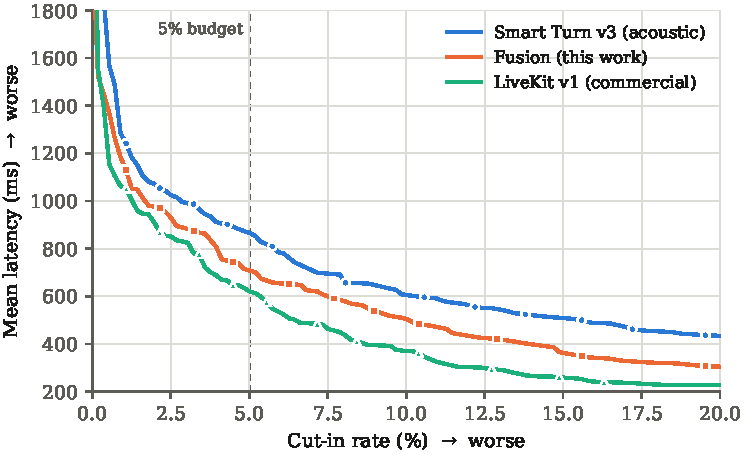
\includegraphics{figures/fig_pareto.pdf}
\caption[Latency against cut-in frontier]{Swept latency-versus-cut-in frontier on the
French benchmark. Lower and to the left is better. The dashed lines mark the 5\,\% and 10\,\% cut-in budgets quoted in
Table~\ref{tab:fusion}.}
\label{fig:pareto}
\end{figure}

\section{Where the gain comes from}
\label{sec:hardcase}

The project is motivated by three cases where silence is a poor cue: a name being spelled
out, digits given in blocks, a pause on a date. It seemed worth checking whether the gain
actually lands on those cases. Each silence was tagged from the causal caller text preceding it, and the AUC recomputed
within each subgroup (Table~\ref{tab:hardcase}).

\begin{table}[H]
\centering
\caption[Per-case breakdown]{Per-case breakdown on the French benchmark. Subgroup sizes
are given first because several groups are far too small to support inference: the spelling
and date rows rest on six and four spans, so their AUCs are reported for completeness only
and no weight is placed on them. Only the digit and plain-text rows are large enough to
compare.}
\label{tab:hardcase}
\begin{tabular}{@{}lrrrcc@{}}
\toprule
Case & $n$ & eot & hold & AUC acoustic & AUC fusion \\
\midrule
Spelling & 6 & 1 & 5 & 0.800 & 1.000 \\
Digits & 269 & 107 & 162 & 0.825 & 0.875 \\
Date & 4 & 2 & 2 & 1.000 & 1.000 \\
Plain text & 764 & 290 & 474 & 0.807 & 0.901 \\
Empty transcript & 11 & 0 & 11 & n/a & n/a \\
\midrule
All & 1{,}054 & 400 & 654 & 0.814 & 0.897 \\
\bottomrule
\end{tabular}
\end{table}

The first of the two findings runs against the framing of this project. On the digit case, which is large
enough to trust at $n = 269$, fusion gains 0.050; on ordinary text it gains 0.094. The motivating case is the one where the lexical signal helps \emph{least}.

That is explicable in hindsight: a partially dictated number is lexically ambiguous in a way an
unfinished sentence is not, because nothing in the words themselves says whether more
digits are coming. The hard cases stay hard, and the bulk of the headline gain comes from
ordinary utterances.

The second is about the benchmark rather than the method itself. Spelling appears six times in
1{,}054 silences and dates four times. Generic French, as sampled here, essentially does not
contain the phenomena that make medical intake difficult, so the public benchmark cannot
test the case the project exists for. This is an argument for in-domain evaluation, not
against it, and it is the reason Section~\ref{sec:gold} matters even though its result is
negative.

\section{Calibration}
\label{sec:calibresults}

Table~\ref{tab:ece} gives the expected calibration error of Equation~\ref{eq:ece}, before
and after post-hoc isotonic recalibration, measured on a held-out split.

\begin{table}[H]
\centering
\caption[Expected calibration error]{Expected calibration error, raw and after post-hoc
isotonic recalibration on a held-out split. Every external system that can be scored at the
evaluation point is listed; nothing is selected. The raw column is the probability each
system actually emits, and the calibrated column is what an integrator can reach by
correcting it, which is available to every row equally.}
\label{tab:ece}
\begin{tabular}{@{}lcc@{}}
\toprule
Model & ECE (raw) & ECE (calibrated) \\
\midrule
Smart Turn v3 & 0.216 & 0.079 \\
ultraVAD & 0.108 & 0.071 \\
LiveKit Turn Detector v1 & 0.091 & 0.052 \\
Deepgram Flux & 0.087 & 0.083 \\
LiveKit Turn Detector v1-mini & 0.084 & 0.051 \\
\midrule
\textbf{This work (fusion)} & \textbf{0.064} & 0.043 \\
\bottomrule
\end{tabular}
\end{table}

The three streaming services are excluded here. An expected calibration error pairs a
predicted probability with the outcome of the same span, which is exactly the pairing
Section~\ref{sec:protocol} rejects for their AUC; reporting one while refusing the other
would be inconsistent. One figure from those excluded runs is worth quoting, not as a result but as evidence for
the exclusion itself: sampled at the evaluation point, GPT-Realtime 2 falls from an ECE of
0.374 to 0.007 under recalibration. A collapse that large is what a near-constant score
looks like, and a system that has not yet decided emits exactly that. No row is given for it
in Table~\ref{tab:ece}.

This chapter treats ECE $> 0.05$ as miscalibrated. The line is a working convention, not a
standard. All five external detectors that can be scored at the evaluation point fall above
it, as do ten of the eleven runs in the span set.
\texttt{calibration\_study.py} in the submitted corpus prints every run.

Before any correction, the fused probability is the best calibrated of the set, at 0.064
against 0.084 for the nearest external system. That is the comparison that bears on
deployment, since none of these systems ships a recalibration step and an integrator
therefore gets the raw column. The margin should not be pressed. v1-mini, Deepgram Flux and LiveKit v1 are all within 0.03,
the table rests on a single held-out split of 214 spans, and no interval is attached to any
of these values. The ordering among the four leading systems is not a result this
dissertation can defend.

The calibrated column does not favour this work. Recalibration needs only a held-out split,
so any integrator can apply it to any row. Applied uniformly it compresses the range:
v1-mini reaches 0.051 and LiveKit v1 0.052 against 0.043 here. The ordering survives, the
distance does not. Across all eleven runs the best-calibrated is this project's own
dialogue-context variant at 0.039, which Section~\ref{sec:negative} reports as a failure on
every other measure. The finding this section supports is therefore about the field and not
about a ranking: miscalibration is universal, correcting it is cheap, and nobody does it.
Nor does that spare this work, which sits uncorrected at 0.064, above the same line.

The mechanism is the one described in Section~\ref{sec:calibration-lit}: these are neural classifiers trained to
discriminate. Nothing in a discriminative objective rewards a probability that matches a
frequency, and the leaderboard never asks for one. 

The consequence is practical. A threshold
placed on a probability that does not correspond to a real frequency cannot be connected to
a cost, and every one of these systems exposes a threshold to its users as though it could
be.

Because isotonic regression is monotonic, this correction moves the probability values
without touching their ordering, which is why none of the AUCs in
Table~\ref{tab:fusion} change under it.

\section{The cost-derived operating point}
\label{sec:costresults}

With a calibrated probability the stopping rule can select its operating point from the
cost ratio $\lambda$ of Equation~\ref{eq:cost}. Table~\ref{tab:cost} shows how the point
moves.

\begin{table}[H]
\centering
\caption{Operating point as a function of the cost ratio
$\lambda = C_{\mathrm{cut}}/C_{\mathrm{lat}}$.}
\label{tab:cost}
\begin{tabular}{@{}lcc@{}}
\toprule
$\lambda$ & Cut-in rate & Latency \\
\midrule
1 (one interruption $=$ 1\,s of latency) & 16.8\,\% & 330\,ms \\
5 & 5.4\,\% & 674\,ms \\
10 & 1.8\,\% & 981\,ms \\
50 (one interruption $=$ 50\,s of latency) & 0.2\,\% & 1525\,ms \\
\bottomrule
\end{tabular}
\end{table}

The endpoint follows from the cost ratio, and the 500\,ms of the existing system appears
nowhere in the calculation. The behaviour is monotone and readable: the more costly an interruption is judged to be, the
more conservative the endpoint becomes.

For medical telephone intake, $\lambda = 10$ is the setting this work would put forward:
1.8\,\% cut-in at 981\,ms. Section~\ref{sec:costdesign} puts the cost of one
interruption at about ten seconds, roughly the length of a repair turn when a caller cut off
mid-identifier has to be asked again. Ten seconds plainly outweighs the 307\,ms saved by
moving to $\lambda = 5$. That rests on judgement: the cost of a repair turn was never
measured, and measuring it on production dialogues is the proper way to fix $\lambda$. What
the framework provides is the means to act on such a cost once known.

How the selected policies reach those points is worth recording, because it bears on the
limits of a threshold rule. The score threshold is not monotone in $\lambda$: across the
four rows it moves 0.37, 0.81, 0.32, 0.46. What does move monotonically is the timing. The
action delay stays at 0.2\,s for $\lambda = 1$ and $5$, then rises to 0.9\,s and 1.0\,s,
and the timeout goes from 1.0\,s to 1.5\,s and then 3.0\,s. At high cost ratios the sweep
buys conservatism by waiting longer, not by demanding a higher score, and it even lowers the
threshold to do so. A rule that only moves a threshold on the current probability cannot
reproduce that, which is what motivates the sequential formulation in
Chapter~\ref{ch:conclusions}.



\section{Negative results}
\label{sec:negative}

Three things were tried and did not work. They are reported because they mark the edges of
the method. The first, a medical-fitted lexical read on generic French, is the 0.789 row of
Table~\ref{tab:fusion} and was discussed in Section~\ref{sec:fusionresults}; the other two
follow.

Folding the elapsed silence into the score did not beat the harness sweep. This variant does not
threshold the acoustic probability directly. It refits $g$ on the acoustic
probability and the silence duration $d$, over the terms $p_{\mathrm{ac}}$, $d$,
$p_{\mathrm{ac}}d$ and $d^{2}$, so one threshold on $g$ acts as a time-varying threshold on
the original score. Applied to the
acoustic baseline it moved the AUC from 0.814 to 0.811. The frontier is bounded by the quality of the score.
The sweep already extracts the best temporal policy, so folding time into the probability
adds nothing it was not already finding.

Augmenting the lexical input with dialogue context did not help either, dropping from 0.897
to 0.854. The completion signal lives in the caller's own words, and mean-pooling frozen
embeddings over the agent's turn as well dilutes it.

On generic French, then, the method plateaus around 0.897. Going
further needs either larger models, outside the scope of this project, or in-domain data,
which the next section tests.

\section{In-domain validation}
\label{sec:gold}

Everything above runs on a clean, generic, public dataset. The in-domain validation uses
French medical calls captured by instrumenting production. Of the 709 calls captured
(Section~\ref{sec:instrumentation}), 636 contribute at least one scored micro-pause. Those
calls yield 5{,}342 micro-pauses: 1{,}015 ends of turn and 4{,}327 holds. The labels come
from weak supervision. The recordings are stereo, caller on the left channel, sampled at 8\,kHz, the
standard telephone band.

Contrary to my hypothesis, fusion does not win in domain. Per pause the AUCs are 0.49 for
the acoustic branch alone, 0.60 for the lexical branch alone and 0.59 for the fusion. The acoustic model is at chance and contributes nothing. Worse for the argument of this
dissertation, fusing is actively harmful here: 0.59 sits below the 0.60 of the lexical
branch on its own, so combining a useful signal with a useless one costs more than it
returns. That is the direct counter-example to the benchmark result of
Section~\ref{sec:fusionresults}, and it holds under the same condition stated there, that
fusion helps only when both inputs carry signal.

Two causes explain this, once bugs are ruled out. The caller channel was confirmed to be the
left one by measuring speech energy in the audio preceding each pause, and both the
timestamp alignment and the scoring point were checked against the benchmark path.

The first cause is bandwidth, and it can be measured rather than assumed. The recordings
are sampled at 8\,kHz, so by Nyquist they carry nothing above 4\,kHz; across sixty of
them, 0.32\,\% of the energy sits above the 3.4\,kHz telephone cut-off and 0.007\,\%
above 4\,kHz. Smart Turn is trained on 16\,kHz wideband, so half the spectrum it learned
on is simply absent.

The effect on its output is visible in the distribution. On the benchmark the score is
spread across the range, with an interquartile range of 0.94 and 41\,\% of spans scored
below 0.1. In domain it collapses against the ceiling: median 0.98, interquartile range
0.09, and 75\,\% of pauses scored above 0.9. The separation between the two classes
disappears with it. On the benchmark the mean score is 0.738 for ends of turn against
0.287 for holds, a gap of $+0.45$; in domain it is 0.820 against 0.844, a gap of
$-0.02$. The model scores holds marginally higher than ends of turn, which is what an
AUC of 0.49 means. A generic acoustic detector does not transfer to 8\,kHz telephony.

The second is the labels. The comparison to draw is between the same lexical branch on the
two datasets. On the public benchmark, where boundaries are human-verified, a frozen
CamemBERT embedding under a logistic head reaches 0.845. The identical construction on the
in-domain set, with labels inferred from resume behaviour, plateaus near 0.60. Nearly a quarter
in absolute AUC separates them, and the only thing that changed is where the labels came
from. Whether a patient resumes speaking is weakly predicted by the words uttered so far,
because a pause followed by a resume and a final pause often have near-identical preceding
text. The ceiling is in the supervision, not in the model.

The per-case breakdown is reported on the public benchmark rather than here. The reason is measurement validity. The in-domain set is roughly five times larger, but with
the acoustic branch at chance and the lexical signal capped at 0.60,
splitting an uninformative measurement by sub-case would yield nothing interpretable. A
breakdown in domain requires the manually annotated subset identified in
Chapter~\ref{ch:conclusions}, which the project timescale did not allow.

So the in-domain validation does not confirm that the method transfers. It shows where it
breaks. This does not contradict the headline result, which stands on clean labels, but it
does show that reaching production takes adaptation. Three directions follow, taken up in
Chapter~\ref{ch:conclusions}: annotate a sample by hand to obtain a clean in-domain test
set; adapt an acoustic model to the 8\,kHz telephone band; rebuild the causal text from
per-turn final transcripts instead of concatenated partial hypotheses.


% ===========================================================================
\cleardoublepage
\chapter{Conclusions and Future Work}
\label{ch:conclusions}

\section{Conclusions}

This project asked a simple question: does adding a semantic signal to an acoustic one, and
then deriving a cost-sensitive decision from the result, improve end-of-turn detection for a
French medical voice agent? On a clean public benchmark the answer is yes. Fusion raises the
AUC from 0.814, for the acoustic model alone, to 0.897, a statistically significant gain of 0.083, and neither base model is fine-tuned in that
pipeline. A medically fine-tuned lexical model exists and serves the in-domain path and the
live demonstration, but it is not what produces this number.

What the project learned is worth as much as what it built. Fusion only helps when the
lexical model is in distribution: applied to generic French, a medically tuned model
degrades the decision below the baseline it was meant to improve. Calibration goes
unreported, though a calibrated probability is the precondition for deciding from a stated
cost rather than an arbitrary timer: every external detector evaluated here is miscalibrated
on this data and none publishes any measurement of it. And the off-the-shelf pipeline does
not transfer to production, for reasons Section~\ref{sec:gold} sets out and O4 returns to.

There is one more finding I did not expect, and it cuts against the framing of the project.
Section~\ref{sec:hardcase} shows the fusion gaining least on precisely the cases the work
exists for, and shows that generic French barely contains those cases at all. The motivating
problem is real, but the public benchmark cannot measure it, and the lexical signal is
weakest exactly where I argued it would be strongest.

This dissertation contributes a calibration-first, cost-aware method for composing existing
models, tested in a real setting, and it measures where that method stops working.

\section{Evaluation against the objectives}

\textbf{O1}, a modular real-time pipeline whose decision never blocks on the transcript, is
met: the package is in place, covered by 45 automated tests, and demonstrated end to end
from the command line and in the browser.

\textbf{O2}, fusing off-the-shelf acoustic and lexical models and testing whether this beats
the acoustic model alone, is met (Section~\ref{sec:fusionresults}).

\textbf{O3}, calibrating the probability and deciding from a cost, is met as analysis and
not as a property of the running system. Calibration was measured across the whole
leaderboard, and the operating point is derived from the cost ratio rather than from a fixed
delay, but that derivation lives in the evaluation: the shipped controller still maps
confidence onto a hand-set silence ladder.

\textbf{O4}, instrumenting production and validating in domain, was carried out, and its
result is negative. The capture and the gold pipeline work, with 709 calls captured and 636 scored, and a validated
converter, but the validation showed that the off-the-shelf pipeline does not transfer: the
acoustic branch is at chance on 8\,kHz audio and the lexical branch plateaus near 0.60 on
weak labels. The objective was delivered as engineering and as measurement; the hypothesis
it was built to test was not confirmed.

Several limitations bound what has been shown. On generic French the method plateaus around
0.897, and passing that needs larger models, which is outside the contribution. The system
trails the commercial streaming services on latency, because it waits for a micro-pause
while they commit as the text arrives. The in-domain labels are weak, and the French
benchmark subset is small at roughly a thousand silences.

There are things I would do differently. I would instrument production in the first week rather
than the seventh, so that a properly annotated in-domain set existed in time instead of a
weakly supervised one. I would check the audio bandwidth of the target deployment before choosing an acoustic
model. The 16\,kHz-to-8\,kHz gap surfaced at validation, which is far too late for it to
surface.
And I would run the per-case breakdown early: had I known in week three that the public
benchmark contains six spelling cases, I would have known from the start that it could not
test the thing the project was for.

The three pillars of this work were set out before implementation began, in the critical
review described in Chapter~\ref{ch:intro}, and two of them survived intact. The third
bent: I evaluate at the micro-pause rather than continuously as speech arrives, which is
exactly the latency gap of Section~\ref{sec:fusionresults} and the first item of future
work below. Being overtaken mid-project was the other thing that shaped the contribution. Narrowing the
claim to calibration and cost, instead of competing on fusion itself, was, I still think,
the right response.

\section{Future work}

The first direction is latency, which is what stands between this system and deployment. It
decides at the micro-pause, which is why it trails services that commit as the text arrives.
Two levers exist: a streaming lexical model that scores word by word and can decide before
the pause, and the stability of the recogniser's interim hypotheses, how quickly the
transcript stops changing, as an early cue. That second signal is only observable in the
partial-hypothesis trajectories captured in production, and cannot be tested on the public
benchmark, which supplies final words only.

The second answers the in-domain result directly: adapt the acoustic model to the 8\,kHz
telephone band, by retraining or by starting from a natively narrowband model, to remove the
saturation, and hand-annotate a few hundred pauses to obtain clean end-of-turn labels and a
trustworthy in-domain measurement, which weak supervision cannot provide.

The third is a sequential optimal-stopping formulation. The current rule applies a myopic
threshold to a calibrated probability. At high cost ratios the swept oracle turns
conservative through timing rather than through the threshold, and a myopic rule cannot
match that. A multi-step cost model, in the tradition of \citet{wald1945sequential}, would
track the oracle across every cost regime.


% ===========================================================================
\appendix
\cleardoublepage
\chapter{Ethics and Data Handling}
\label{app:ethics}

\section{Context and partnership}

This project was carried out in partnership with Tennor, which operates a French medical
voice agent that patients call by telephone. The work builds a real-time end-of-utterance
detector for that agent. Tennor is the data controller and operates a GDPR-compliant,
ISO/IEC 27001-certified environment. I processed the data inside Tennor's infrastructure as
part of the partnership. No participants were recruited and there was no interaction with
patients: the work reuses signals already generated by the live system.

\medskip
\noindent\fbox{\parbox{0.95\textwidth}{\small
\textbf{Correction to the statement submitted with the corpus.} The ethics statement
submitted alongside the code corpus on 21 August 2026 describes the capture as limited to
\emph{internal test organisations}. That is narrower than what actually happened: capture
was feature-flag gated at organisation level on \emph{production} organisations. This
appendix supersedes that statement and gives the accurate position. The correction was
raised with my supervisor before writing. The corpus itself can no longer be amended.}}

\section{Data used}

\textbf{Public benchmark, no personal data.} Every headline result reported in
Chapter~\ref{ch:results} runs on the LiveKit eot-bench dataset (CC-BY-4.0), a public French
turn-taking benchmark containing no Tennor data and no personal data. The benchmark
deliberately carries the weight of the evaluation, so that the method can be demonstrated
without personal data at all (Section~\ref{sec:datastrategy}).

\textbf{Production in-domain set.} A secondary, in-domain set was derived from calls to the
Tennor agent: 709 calls placed on a single production organisation, of which roughly four in five
are genuine inbound calls and the remainder calls made by internal testers to the same line.
It is used only as an in-domain validation set, and it is not included in the corpus.

\section{Legal basis and agreement with the controller}

Tennor is the data controller. Every use of Tennor data in this project was agreed with the
company before it took place, and the company reviewed the scope of the capture, the fields
retained, this appendix, and the dissertation itself. Tennor is aware of what the work covers
and of what it implies for the production agent. Nothing was collected, processed, or released
outside that agreement, and the partnership was conducted transparently on both sides.

One consequence follows directly. The in-domain production set described above, referred to as
the \emph{gold} set in the submitted corpus, cannot be shared or made public. The reason is data
sovereignty: these are French medical call recordings and transcripts held in Tennor's own
infrastructure, and they stay there. The set is therefore described and measured in this
dissertation but not distributed with it, which is why the public benchmark carries every
headline result (Section~\ref{sec:datastrategy}).

\section{Pseudonymisation, not anonymisation}

Names, first names and ages are masked in the retained transcripts, and the export is
reduced to the fields the task uses. The data nonetheless remains personal data under the GDPR: the caller-side audio is
retained and every record is linked to a production call identifier, so re-identification by
the controller remains possible. It is treated as personal data throughout, and describing
it as anonymised would be incorrect. The fields the task uses are the caller text, the recogniser's interim trajectory, the pause
and decision timestamps, an audio reference, and the resume and interruption flags. The
export is reduced to these.

\section{Reduced human exposure}

Labels are produced automatically by weak supervision, from whether the caller resumed
speaking after a pause (Section~\ref{sec:instrumentation}). Building the dataset therefore
required nobody to sit and listen to call content, which limits human exposure to what
patients said. The cost of that choice is label noise, and it bounds the result reported in
Section~\ref{sec:gold}. It is an ethical decision with a measurable methodological price,
which is worth stating in both directions.

\section{Storage, access and the corpus}

The data and any derived audio or transcripts stay within Tennor's infrastructure. Access
was restricted to me. Nothing was copied into the repository, the corpus, or any public
location: \texttt{.gitignore} excludes call audio, transcripts and model weights, and the
corpus was packaged and checked so that none of those files were included. The corpus
contains the source code, the dataset-generation code, the evaluation on the public dataset,
the design documents and this statement.

\section{Risks and mitigations}

\begin{table}[H]
\centering
\small
\begin{tabular}{@{}p{5.5cm}p{8.0cm}@{}}
\toprule
Risk & Mitigation \\
\midrule
Exposure of patient data & Nothing leaves Tennor's infrastructure; no audio, transcript or
derived record in the corpus; access limited to the author \\
Re-identification & Names, first names and ages masked in the retained transcripts; treated as personal data throughout rather than described as anonymised; nothing exported beyond Tennor's infrastructure \\
Accidental inclusion in the corpus & \texttt{.gitignore} rules plus packaging that excludes
audio, transcripts and weights, verified before submission \\
Over-collection & Only caller-side, task-relevant fields captured per micro-pause \\
Human exposure to call content & Automatic weak-supervision labelling instead of manual
listening \\
Clinical impact of a wrong cut & Cost-sensitive decision with the interruption cost stated
explicitly, and cut-in rates reported openly; the system augments rather than replaces
existing safeguards \\
\bottomrule
\end{tabular}
\end{table}


\cleardoublepage
\bibliographystyle{kentHarvard}
\cleardoublepage
\bibliography{diss}

\end{document}
